\documentclass[11pt]{article}
\usepackage[margin=0.75in]{geometry}
\usepackage{amsmath,amssymb,graphicx,hyperref}
\setlength{\parindent}{0pt}\setlength{\parskip}{4pt}
\setlength{\emergencystretch}{3em}
\begin{document}
{\Large Public norm jets and coupled branch reconstruction}\par
2026-11-13. Unsigned producer evidence [pcc:unverified].

\textbf{Question.} Can explicit node-preserving polynomial jets correct a norm
while retaining the pole-degree window? This round tests a specified polynomial
family, without claiming it represents the older matrix $W$-family.

\textbf{Exact map.} Put $N(A,B)=A^2-fB^2$, $A'=A+GJ$, $B'=B+GK$. Then
\[
 N(A',B')=N(A,B)+G(2AJ-2fBK)+G^2(J^2-fK^2).
\]
For $2u=1$ and $AU+fBV+GW=1$, take $J=uU\Delta$, $K=-uV\Delta$. Exactly
\[
 N(A',B')-N(A,B)-G\Delta=G^2(J^2-fK^2-W\Delta).
\]
Every first quotient jet is reachable with the explicit inverse, but the full
residual is retained. This is classical Hensel algebra [pcc:unverified].

\textbf{Actual degree constraint.} If old and new coordinate degrees are all
strictly below $\deg G$, differences divisible by $G$ are zero. Thus $J=K=0$
when $G\ne0$. The actual pole bounds $2\deg A\le\deg G$ and
$\deg f+2\deg B\le\deg G$ imply those strict bounds when $\deg G>0$.
Componentwise jets cannot produce a new target norm inside that window.
This conclusion does not exclude coupled or rational operations [pcc:unverified].

\begin{center}
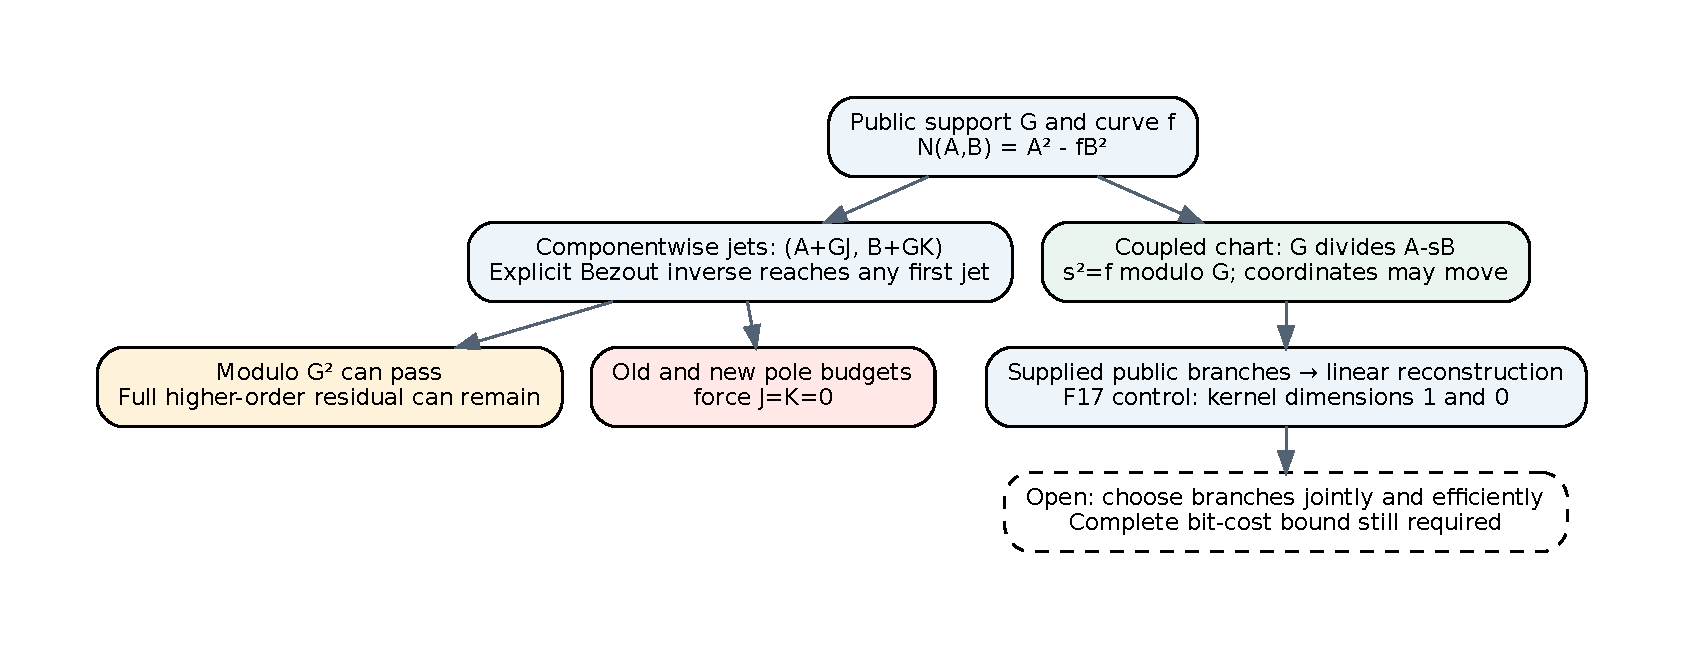
\includegraphics[width=0.92\linewidth,height=0.39\textheight,keepaspectratio]{jets.pdf}
\end{center}

\textbf{Coupled successor.} Fix $s$ with $G\mid s^2-f$. Changes
$(A+sH+GJ,B+H)$ preserve $A-sB$ modulo $G$ while individual coordinates can
move. Since
\[
 A^2-fB^2=(A-sB)(A+sB)+(s^2-f)B^2,
\]
branch congruence gives norm divisibility. Monic $G$, actual pole bounds and
nonzero norm then give $N=CcG$ for $c\ne0$, without moments or cofactors.
Choosing the root branches and finding the bounded pair remain inputs
[pcc:unverified].

\newpage
{\Large Fixed controls, proof scope and next finder obligation}\par
\textbf{Local versus exact.} One write-once native fixture tests all289
$\Delta$ of degree at most1 over F17, with $f=X^3+2X+2$, $G=X$, $A=6$,
$B=1$, $V=9$, $W=16+8X^2$. Exactly288 retain a nonzero full residual.
For target $c=1$, the public lift gives
\[
 B'=1+12X+4X^3,\qquad
 N(6,B')-G=4X^2+X^3+6X^4+4X^5+11X^6+8X^7+X^9.
\]
It passes modulo $G^2$, but fails the exact norm and degree window. This is an
algebra fixture of support degree1, not a cubic ECDLP relation instance.
Coefficient identities, node/derivative values and all17 point evaluations
are checked; cases are deterministic, not independent trials [pcc:unverified].

\textbf{Public branch reconstruction.} From the supplied public points
$(0,6),(3,1),(5,1),(6,3),(10,11),(13,7)$, construct $s$ by Lagrange interpolation
and solve the six original homogeneous equations for $\deg A\le3$, $\deg B\le1$.
No known $A/B$ is supplied to that solve. Check original rows, point equations,
branch congruence, degree bounds and full norm identity [pcc:unverified].
\begin{center}\small
\begin{tabular}{lll}
Supplied assignment & Kernel dimension & Result\\\hline
Six points above &1&$A=[14,2,7,3],\ B=[8,1],\ c=9$\\
Only $(13,7)\to(13,10)$ &0&No bounded nonzero pair for these branches
\end{tabular}
\end{center}
The positive pair is3 times the original fixture pair, with norm scaling9.
The flipped result concerns one sign assignment; it does not exclude the
unsigned support, whose positive assignment is exhibited. This is supplied-branch
reconstruction, not branch selection or an attack search [pcc:unverified].

\textbf{Formalization.} Fourteen new statements in \path{NormPublicJets.lean};
source \path{8892e4477}, final native source \path{a5b04b3e5}. Whole-study
tracked-source gate:231 statements,0 additional trusted axioms. Explicit
kernel replay receipts and source hashes accompany the report. Lean4.35.0,
CryptoLean\path{148f5dc389b}, Mathlib\path{cfc55fc58714}. Initial build001
failed on a lemma invocation;002 passes. Strict clippy001 failed on an indexed
loop;002 passes after an actual repair, with7 tests passing. All failures and
exact exits remain [pcc:unverified].

\textbf{Source claims, unsigned.}\par
First jet: \path{PCC-20261113-4969cb}.\par
Actual-window implication: \path{PCC-20261113-f8bb46}.\par
Coupled certificate: \path{PCC-20261113-41d872}.\par
Native fixture: \path{PCC-20261113-e63c86}.\par
The full14-statement proof map and claim pins are in the source-linked README.
Default-PATH source-only PCC checks are not\_covered, distinct from the
explicit-toolchain kernel checks. No signed verdict is supplied.

\textbf{Next obligation.} Efficiently select square-root branches jointly with
bounded reconstruction, with all rejected attempts and setup charged. Keep
$\exp(o(\log r))$ complete bit cost on general prime curves as the acceptance
criterion. The finite linear solve does not discharge branch selection
[pcc:unverified].

\textbf{Prior art.} Galbraith, \emph{Mathematics of Public Key Cryptography},
2.13 (Hensel expansion),8.4 (Riemann--Roch/pole constraints), cached primary
text; previous norm derivation and recovery source. KB MCP unavailable;
canonical wrapper exits127 (no executable). No exhaustive or novelty claim.
\end{document}
